%%%%%%%%%%%%%%%%%%%%%%%%%%%%%%%%%%%%%%%%%
% University/School Laboratory Report
% LaTeX Template
% Version 4.0 (March 21, 2022)
%
% This template originates from:
% https://www.LaTeXTemplates.com
%
% Authors:
% Vel (vel@latextemplates.com)
% Linux and Unix Users Group at Virginia Tech Wiki
%
% License:
% CC BY-NC-SA 4.0 (https://creativecommons.org/licenses/by-nc-sa/4.0/)
%
%%%%%%%%%%%%%%%%%%%%%%%%%%%%%%%%%%%%%%%%%

%----------------------------------------------------------------------------------------
%	PACKAGES AND DOCUMENT CONFIGURATIONS
%----------------------------------------------------------------------------------------

\documentclass[
	letterpaper, % Paper size, specify a4paper (A4) or letterpaper (US letter)
	10pt, % Default font size, specify 10pt, 11pt or 12pt
]{CSUniSchoolLabReport}

%----------------------------------------------------------------------------------------
%	REPORT INFORMATION
%----------------------------------------------------------------------------------------

\title{ECE 398-MA \\ Introduction to Modern Communication with Python and SDR \\ ADI Pluto SDR Lab 2 -- FM Transceiver} % Report title

\author{Noah Breit} % Author name(s), add additional authors like: '\& James \textsc{Smith}'

\date{\today} % Date of the report

%----------------------------------------------------------------------------------------

\begin{document}

\maketitle % Insert the title, author and date using the information specified above

% \begin{center}
% 	\begin{tabular}{l r}
% 		Date Performed: & February 13, 2022 \\ % Date the experiment was performed
% 		Partners: & Cecilia \textsc{Smith} \\ % Partner names
% 		& Tajel \textsc{Khumalo} \\
% 		Instructor: & Professor \textsc{Rivera} % Instructor/supervisor
% 	\end{tabular}
% \end{center}

% If you need to include an abstract, uncomment the lines below
%\begin{abstract}
%	Abstract text
%\end{abstract}

%----------------------------------------------------------------------------------------
%	OBJECTIVE
%----------------------------------------------------------------------------------------

\section{Assignment 1}

\begin{lstlisting}[language=Python]
	import numpy as np
	import matplotlib.pyplot as plt
	from scipy.io import wavfile
	from scipy.signal import butter, filtfilt
	
	# Load stereo audio file
	path_to_file = 'stereo.wav'  # Update this path
	fs_audio, audio = wavfile.read(path_to_file)
	
	# Extract Left and Right audio channels
	audio_L = audio[:, 0]
	audio_R = audio[:, 1]
	
	# Time vector for original audio
	t_audio = np.arange(len(audio_L)) / fs_audio
	
	# Anti-Aliasing Low-Pass Filter (LPF) @ fs_audio (0-15 kHz)
	Nfilt = 5
	cutoff = 15e3
	b_AAF, a_AAF = butter(Nfilt, cutoff / (fs_audio / 2), btype='low')
	
	# Apply LPF to L and R audio signals
	audio_L_filt = filtfilt(b_AAF, a_AAF, audio_L)
	audio_R_filt = filtfilt(b_AAF, a_AAF, audio_R)
	
	# Plot time-domain samples of the Left and Right channels
	plt.figure(figsize=(10, 4))
	plt.subplot(121)
	plt.plot(t_audio, audio_L, label='Original Left Channel')
	plt.plot(t_audio, audio_L_filt, label='Filtered Left Channel')
	plt.xlabel('Time (s)')
	plt.ylabel('Amplitude')
	plt.title('Time-Domain Samples of Left Channel')
	plt.legend()
	
	plt.subplot(122)
	plt.plot(t_audio, audio_R, label='Original Right Channel')
	plt.plot(t_audio, audio_R_filt, label='Filtered Right Channel')
	plt.xlabel('Time (s)')
	plt.ylabel('Amplitude')
	plt.title('Time-Domain Samples of Right Channel')
	plt.legend()
	plt.tight_layout()
	plt.savefig('assignment1a.png')
	plt.show()
	
	# Plot log-scale spectrum of the original and filtered Left-channel audio
	plt.figure(figsize=(10, 4))
	plt.subplot(121)
	plt.semilogy(np.abs(np.fft.fftshift(np.fft.fft(audio_L))), label='Original Left Channel')
	plt.xlabel('Frequency Bin')
	plt.ylabel('Magnitude')
	plt.title('Log-Scale Spectrum of Original Left Channel')
	plt.legend()
	
	plt.subplot(122)
	plt.semilogy(np.abs(np.fft.fftshift(np.fft.fft(audio_L_filt))), label='Filtered Left Channel')
	plt.xlabel('Frequency Bin')
	plt.ylabel('Magnitude')
	plt.title('Log-Scale Spectrum of Filtered Left Channel')
	plt.legend()
	plt.tight_layout()
	plt.savefig('assignment1b.png')
	plt.show()
	
\end{lstlisting}

\begin{figure}[H] % [H] forces the figure to be placed exactly where it appears in the text
	\centering % Horizontally center the figure
	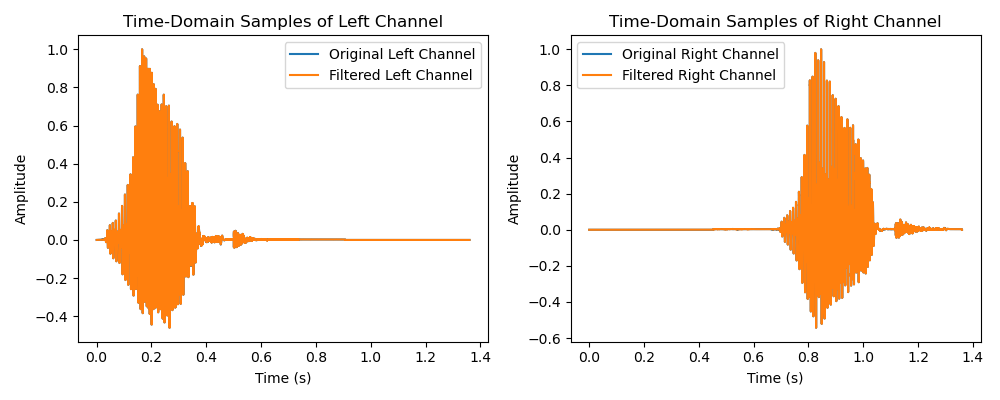
\includegraphics[width=1.2\textwidth]{assignment1a.png} % Include the figure
	\caption{Time-Domain Left-Right Signals}
	\label{fig:block}
\end{figure}

\begin{figure}[H] % [H] forces the figure to be placed exactly where it appears in the text
	\centering % Horizontally center the figure
	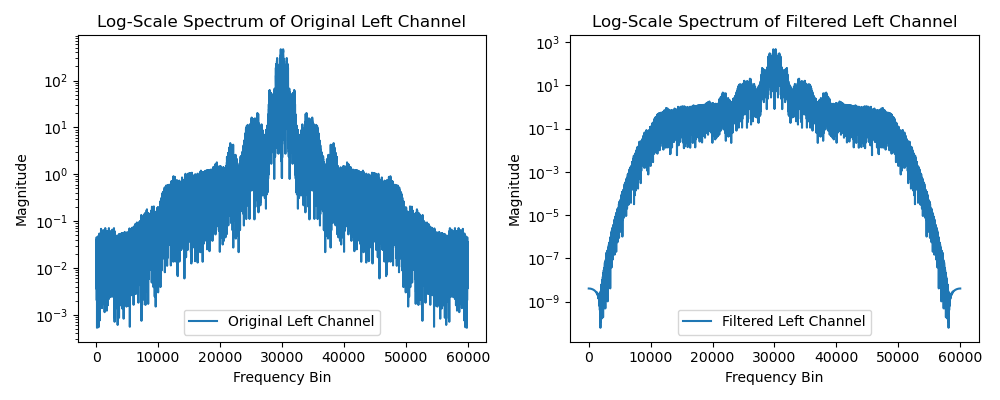
\includegraphics[width=1.2\textwidth]{assignment1b.png} % Include the figure
	\caption{Log-Scale Spectrum Left-Right Signals}
	\label{fig:block}
\end{figure}

\section{Assignment 2}

\begin{lstlisting}[language=Python]
	import numpy as np
	import matplotlib.pyplot as plt
	from scipy.io import wavfile
	from scipy.signal import butter, filtfilt, resample_poly
	
	# Load stereo audio file
	path_to_file = 'stereo.wav'  # Update this path
	fs_audio, audio = wavfile.read(path_to_file)
	
	# Extract Left and Right audio channels
	audio_L = audio[:, 0]
	audio_R = audio[:, 1]
	
	# Time vector for original audio
	t_audio = np.arange(len(audio_L)) / fs_audio
	
	# Anti-Aliasing Low-Pass Filter (LPF) @ fs_audio (0-15 kHz)
	Nfilt = 5
	cutoff = 15e3
	b_AAF, a_AAF = butter(Nfilt, cutoff / (fs_audio / 2), btype='low')
	
	# Apply LPF to L and R audio signals
	audio_L_filt = filtfilt(b_AAF, a_AAF, audio_L)
	audio_R_filt = filtfilt(b_AAF, a_AAF, audio_R)
	
	########### PART 2 ###########
	
	# Upsample audio to PlutoSDR sampling rate
	M = 15
	fs = M * fs_audio  # PlutoSDR sampling rate
	mL = resample_poly(audio_L_filt, M, 1)
	mR = resample_poly(audio_R_filt, M, 1)
	
	# Time vector for resampled audio
	N = len(mL)
	t = np.arange(N) / fs
	
	# Pilot Signal
	fp = 19e3  # Pilot frequency
	ap = 0.1  # Pilot amplitude
	pilot = ap * np.cos(2 * np.pi * fp * t)
	
	# DSB-SC Modulated (L-R) Signal
	DSB_carrier = np.cos(2 * np.pi * 2 * fp * t)
	mLmR_dsb = (mL - mR) * DSB_carrier
	
	# Composite Message Signal m(t)
	mTx = (mL + mR) + pilot + mLmR_dsb
	
	# Normalize message signal
	mTx /= np.max(np.abs(mTx))
	
	# Plot time-domain samples of m(t)
	plt.figure(figsize=(10, 4))
	plt.plot(t, mTx)
	plt.xlabel('Time (s)')
	plt.ylabel('Amplitude')
	plt.title('Time-Domain Samples of Message Signal m(t)')
	plt.savefig('assignment2a.png')
	plt.show()
	
	# Plot log-scale spectrum of m(t)
	plt.figure(figsize=(10, 4))
	plt.semilogy(np.abs(np.fft.fftshift(np.fft.fft(mTx))))
	plt.xlabel('Frequency Bin')
	plt.ylabel('Magnitude')
	plt.title('Log-Scale Spectrum of Message Signal m(t)')
	plt.savefig('assignment2b.png')
	plt.show()

\end{lstlisting}

\begin{figure}[H] % [H] forces the figure to be placed exactly where it appears in the text
	\centering % Horizontally center the figure
	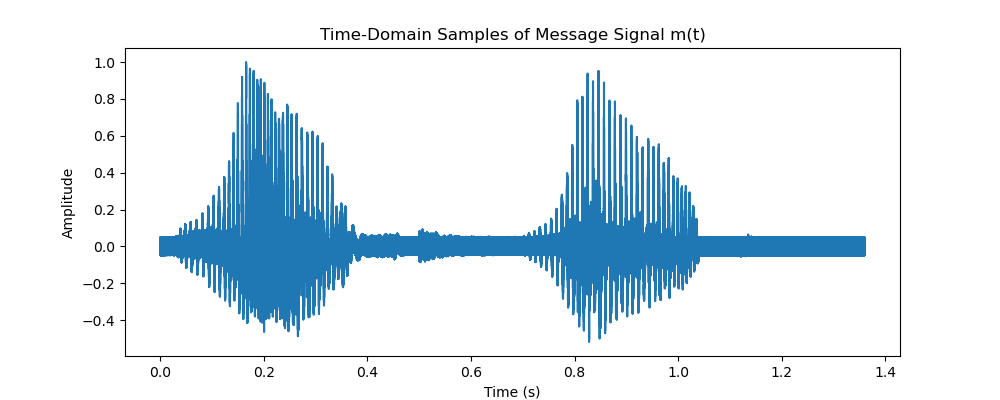
\includegraphics[width=1.2\textwidth]{assignment2a.png} % Include the figure
	\caption{Time-Domain Samples of M(t)}
	\label{fig:block}
\end{figure}

\begin{figure}[H] % [H] forces the figure to be placed exactly where it appears in the text
	\centering % Horizontally center the figure
	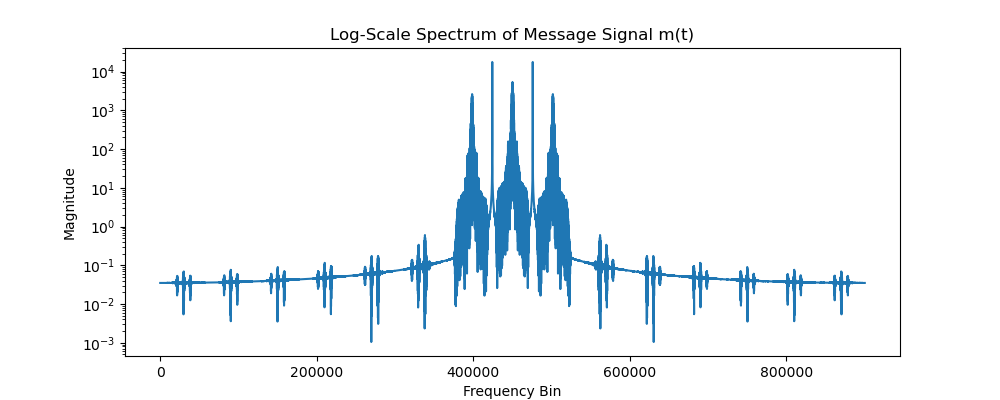
\includegraphics[width=1.2\textwidth]{assignment2b.png} % Include the figure
	\caption{Log-Scale Spectrum of M(t)}
	\label{fig:block}
\end{figure}

\section{Assignment 3}

\begin{lstlisting}[language=Python]
	######### PART 3 #############
	
	### REUSING ASSIGNMENT 2 CODE ABOVE ###
	
	# FM Modulation Parameters
	fc = 100e6  # Carrier frequency
	kf = 75e3  # Frequency deviation
	
	# Compute the instantaneous phase
	phase = 2 * np.pi * kf * np.cumsum(mTx) / fs
	
	# Complex baseband signal
	x_t = np.exp(1j * phase)
	
	# Plot the phase phi(t)
	plt.figure(figsize=(10, 4))
	plt.plot(t, phase)
	plt.xlabel('Time (s)')
	plt.ylabel('Phase (rad)')
	plt.title('Phase of FM Modulated Signal')
	plt.savefig('assignment3a.png')
	plt.show()
	
	# Plot the log-scale spectrum of x(t)
	plt.figure(figsize=(10, 4))
	plt.semilogy(np.abs(np.fft.fftshift(np.fft.fft(x_t))))
	plt.xlabel('Frequency Bin')
	plt.ylabel('Magnitude')
	plt.title('Log-Scale Spectrum of Complex Baseband Signal')
	plt.savefig('assignment3b.png')
	plt.show()

\end{lstlisting}

\begin{figure}[H] % [H] forces the figure to be placed exactly where it appears in the text
	\centering % Horizontally center the figure
	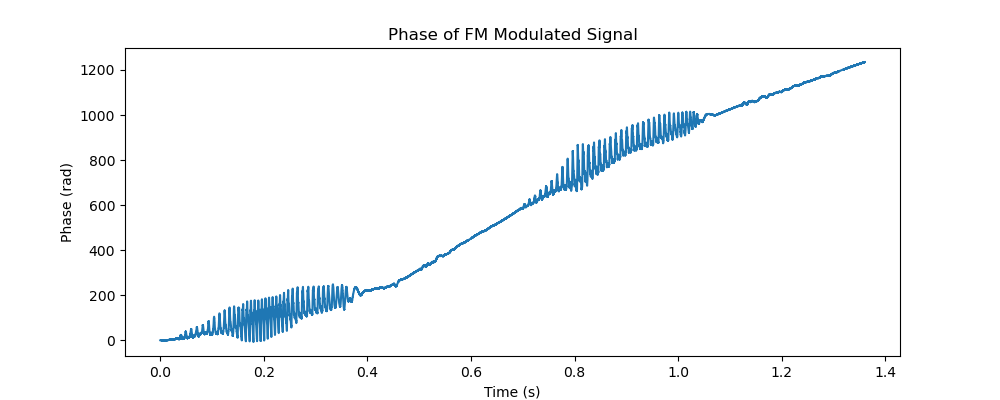
\includegraphics[width=1.2\textwidth]{assignment3a.png} % Include the figure
	\caption{Time-Domain PHI(t) Signal}
	\label{fig:block}
\end{figure}

\begin{figure}[H] % [H] forces the figure to be placed exactly where it appears in the text
	\centering % Horizontally center the figure
	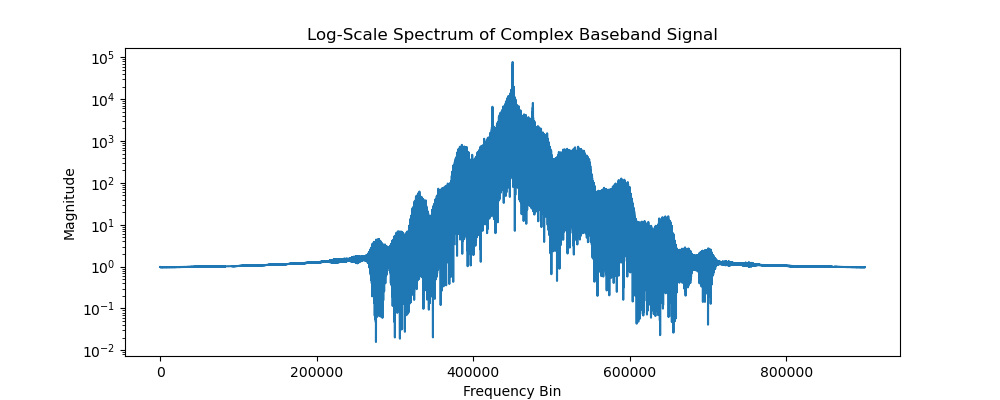
\includegraphics[width=1.2\textwidth]{assignment3b.png} % Include the figure
	\caption{Log-Scale Spectrum of X(t)}
	\label{fig:block}
\end{figure}

\section{Assignment 4}

\begin{lstlisting}[language=Python]
	import numpy as np
	import matplotlib.pyplot as plt
	from scipy.io import wavfile
	from scipy.signal import butter, filtfilt, resample_poly, hilbert
	import adi
	
	# Load stereo audio file
	path_to_file = 'stereo.wav'
	fs_audio, audio = wavfile.read(path_to_file)
	
	# Extract Left and Right audio channels
	audio_L = audio[:, 0]
	audio_R = audio[:, 1]
	
	# Time vector for original audio
	t_audio = np.arange(len(audio_L)) / fs_audio
	
	# Anti-Aliasing Low-Pass Filter (LPF) @ fs_audio (0-15 kHz)
	Nfilt = 5
	cutoff = 15e3
	b_AAF, a_AAF = butter(Nfilt, cutoff / (fs_audio / 2), btype='low')
	
	# Apply LPF to L and R audio signals
	audio_L_filt = filtfilt(b_AAF, a_AAF, audio_L)
	audio_R_filt = filtfilt(b_AAF, a_AAF, audio_R)
	
	# Upsample audio to PlutoSDR sampling rate
	M = 15
	fs = M * fs_audio  # PlutoSDR sampling rate
	mL = resample_poly(audio_L_filt, M, 1)
	mR = resample_poly(audio_R_filt, M, 1)
	
	# Time vector for resampled audio
	N = len(mL)
	t = np.arange(N) / fs
	
	# Pilot Signal
	fp = 19e3  # Pilot frequency
	ap = 0.1  # Pilot amplitude
	pilot = ap * np.cos(2 * np.pi * fp * t)
	
	# DSB-SC Modulated (L-R) Signal
	DSB_carrier = np.cos(2 * np.pi * 2 * fp * t)
	mLmR_dsb = (mL - mR) * DSB_carrier
	
	# Composite Message Signal m(t)
	mTx = (mL + mR) + pilot + mLmR_dsb
	
	# Normalize message signal
	mTx /= np.max(np.abs(mTx))
	
	# FM Modulation Parameters
	fc = 100e6  # Carrier frequency
	kf = 75e3  # Frequency deviation
	
	# Compute the instantaneous phase
	phase = 2 * np.pi * kf * np.cumsum(mTx) / fs
	
	# Complex baseband signal
	x_t = np.exp(1j * phase)
	
	###### SETUP ADI PLUTO SDR ###########
	
	# Set SDR parameters
	sdr_carrier_freq = 100e6  # Carrier frequency (Hz)
	sdr_tx_gain = -50.0  # Tx gain (-90 to 0 dB)
	sdr_rx_gain = 50.0   # Rx gain (0 to 74.5 dB) - Adjust to avoid ADC saturation
	
	# Create PlutoSDR object
	sdr = adi.Pluto("ip:192.168.2.1")
	
	# Configure common settings
	sdr.sample_rate = int(fs)
	sdr.gain_control_mode_chan0 = 'manual'
	
	# Configure Tx
	sdr.tx_rf_bandwidth = int(fs)  # Set Tx filter cutoff to match sample rate
	sdr.tx_lo = int(sdr_carrier_freq)
	sdr.tx_hardwaregain_chan0 = sdr_tx_gain  # Adjust Tx power (-90 to 0 dB)
	
	# Configure Rx
	sdr.rx_lo = int(sdr_carrier_freq)
	sdr.rx_rf_bandwidth = int(fs)
	sdr.rx_buffer_size = int(N)  # Buffer size for Rx samples
	sdr.rx_hardwaregain_chan0 = sdr_rx_gain  # Adjust Rx gain (0 to 74.5 dB)
	
	# Echo SDR configuration
	print("sample_rate (MHz):", sdr.sample_rate * 1e-6)
	print("tx_lo (MHz):", sdr.tx_lo * 1e-6)
	print("tx_rf_bandwidth (MHz):", sdr.tx_rf_bandwidth * 1e-6)
	print("tx_hardwaregain_chan0 (dB):", sdr.tx_hardwaregain_chan0)
	print("rx_lo (MHz):", sdr.rx_lo * 1e-6)
	print("rx_rf_bandwidth (MHz):", sdr.rx_rf_bandwidth * 1e-6)
	print("rx_buffer_size:", sdr.rx_buffer_size)
	print("rx_hardwaregain_chan0 (dB):", sdr.rx_hardwaregain_chan0)
	
	###### TRANSMIT MODULATED FM TRANSMISSION ########
	
	# Scale complex baseband signal to SDR expected range
	tx_samples = x_t * 2**14  
	
	# Enable cyclic buffer and start transmission
	sdr.tx_cyclic_buffer = True
	sdr.tx(tx_samples)
	
	############## DEMOD FM TRANSMISSION ################
	
	# Clear buffer before capturing data
	for _ in range(3):
	sdr.rx()
	
	# Capture two consecutive frames of received data
	frame1 = sdr.rx()
	raw_data = 2**-14 * frame1  # Scale back to (-1,1) range
	
	# Apply 53 kHz LPF to remove out-of-band noise
	Nfilt_rf = 11
	cutoff_rf = 53e3
	b_LPF_rf, a_LPF_rf = butter(Nfilt_rf, cutoff_rf / (fs / 2), btype='low')
	filtered_data = filtfilt(b_LPF_rf, a_LPF_rf, raw_data)
	
	# Extract phase from the complex signal
	phase_rx = np.unwrap(np.angle(filtered_data))
	
	# Compute the FM demodulated message signal
	mRx = (phase_rx[1:] - phase_rx[:-1]) * fs / (2 * np.pi * kf)
	mRx = np.append(mRx, mRx[-1])  # Append a zero to match the original length
	
	# Plot the demodulated message signal m(t) in the time domain
	plt.figure(figsize=(10, 4))
	plt.plot(t, mRx)
	plt.xlabel('Time (s)')
	plt.ylabel('Amplitude')
	plt.title('Demodulated Message Signal m(t)')
	plt.savefig('assignment4a.png')
	plt.show()
	
	# Plot the log-scale spectrum of m(t)
	plt.figure(figsize=(10, 4))
	plt.semilogy(np.abs(np.fft.fftshift(np.fft.fft(mRx))))
	plt.xlabel('Frequency Bin')
	plt.ylabel('Magnitude')
	plt.title('Log-Scale Spectrum of Demodulated Message Signal')
	plt.savefig('assignment4b.png')
	plt.show()
	
\end{lstlisting}

\begin{figure}[H] % [H] forces the figure to be placed exactly where it appears in the text
	\centering % Horizontally center the figure
	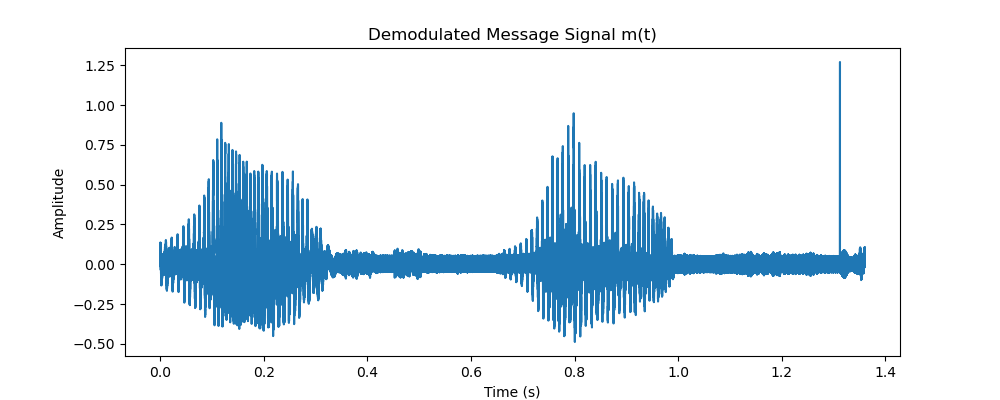
\includegraphics[width=1.2\textwidth]{assignment4a.png} % Include the figure
	\caption{Demodulated FM signal M(t) in Time-Domain}
	\label{fig:block}
\end{figure}

\begin{figure}[H] % [H] forces the figure to be placed exactly where it appears in the text
	\centering % Horizontally center the figure
	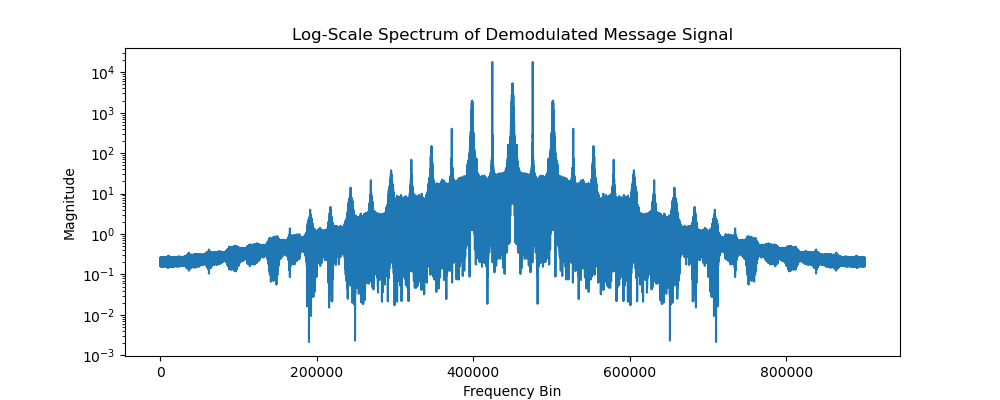
\includegraphics[width=1.2\textwidth]{assignment4b.png} % Include the figure
	\caption{Log-Scale Spectrum of M(t)}
	\label{fig:block}
\end{figure}

\section{Assignment 5}

\begin{lstlisting}[language=Python]
	########## EXTRACT AUDIO FROM DEMOD FM TRANSMISSION ################
	
	# Extract Audio Components
	# Low-pass filter for L+R audio (0-15 kHz)
	Nfilt_audio = 9
	cutoff_audio = 15e3
	b_LPF_audio, a_LPF_audio = butter(Nfilt_audio, cutoff_audio / (fs / 2), btype='low')
	L_plus_R = filtfilt(b_LPF_audio, a_LPF_audio, mRx)
	
	# Narrowband filter for pilot tone (19 kHz)
	Nfilt_band = 5
	cutoff_band_pilot = [18e3, 20e3]
	b_narrow, a_narrow = butter(Nfilt_band, np.array(cutoff_band_pilot) / (fs / 2), btype='band')
	pilot_rx = filtfilt(b_narrow, a_narrow, mRx)
	
	# Band-pass filter for DSB-SC carrier (38 kHz)
	cutoff_band_dsb = [23e3, 53e3]
	b_BPF, a_BPF = butter(Nfilt_band, np.array(cutoff_band_dsb) / (fs / 2), btype='band')
	DSB_carrier_rx = filtfilt(b_BPF, a_BPF, mRx)
	
	# Extract phase of the recovered pilot using Hilbert transform
	pilot_phase = np.unwrap(np.angle(hilbert(pilot_rx)))
	
	# Double the phase to obtain the DSB-SC carrier
	DSB_carrier_phase = 2 * pilot_phase
	
	# Recover the difference signal (L-R)
	L_minus_R = DSB_carrier_rx * np.cos(DSB_carrier_phase) * 2
	
	# Recover Left and Right channels
	L_audio = (L_plus_R + L_minus_R) / 2
	R_audio = (L_plus_R - L_minus_R) / 2
	
	# Downsample audio back to 44.1 kHz
	L_audio_downsampled = resample_poly(L_audio, 1, M)
	R_audio_downsampled = resample_poly(R_audio, 1, M)
	
	# Plot the first 200 samples of the pilot signal
	plt.figure(figsize=(10, 4))
	plt.plot(pilot_rx[:200])
	plt.xlabel('Sample Index')
	plt.ylabel('Amplitude')
	plt.title('First 200 Samples of Pilot Signal')
	plt.savefig('assignment5a.png')
	plt.show()
	
	# Plot the first 200 samples of the DSB-SC carrier signal
	plt.figure(figsize=(10, 4))
	plt.plot(DSB_carrier_rx[:200])
	plt.xlabel('Sample Index')
	plt.ylabel('Amplitude')
	plt.title('First 200 Samples of DSB-SC Carrier Signal')
	plt.savefig('assignment5b.png')
	plt.show()
	
	# Plot the recovered Left and Right audio signals in the time domain
	plt.figure(figsize=(10, 4))
	plt.subplot(121)
	plt.plot(L_audio_downsampled)
	plt.xlabel('Time (s)')
	plt.ylabel('Amplitude')
	plt.title('Recovered Left Audio')
	plt.subplot(122)
	plt.plot(R_audio_downsampled)
	plt.xlabel('Time (s)')
	plt.ylabel('Amplitude')
	plt.title('Recovered Right Audio')
	plt.tight_layout()
	plt.savefig('assignment5c.png')
	plt.show()
	
	# Save the recovered stereo audio as a WAV file
	from scipy.io.wavfile import write
	
	stereo_demod = np.column_stack((L_audio_downsampled, R_audio_downsampled))
	stereo_demod_int16 = (stereo_demod * 32767).astype(np.int16)  # Convert to 16-bit PCM
	write("recovered_stereo.wav", int(fs_audio), stereo_demod_int16)
	
\end{lstlisting}

\begin{figure}[H] % [H] forces the figure to be placed exactly where it appears in the text
	\centering % Horizontally center the figure
	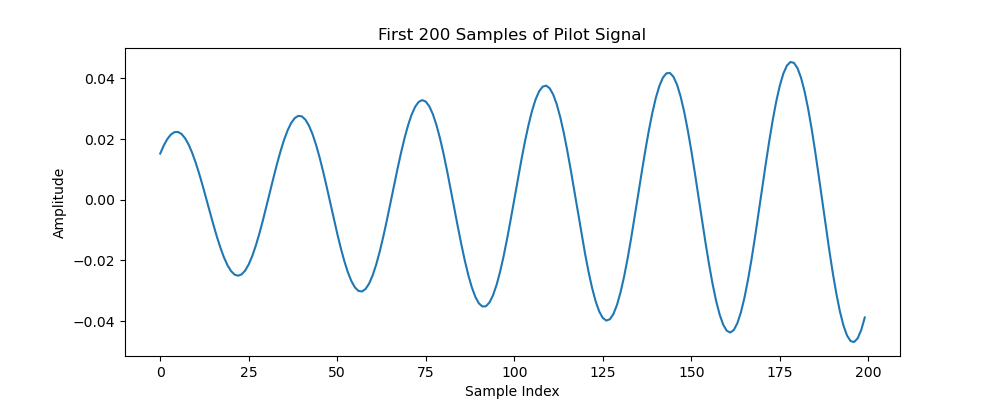
\includegraphics[width=1.2\textwidth]{assignment5a.png} % Include the figure
	\caption{First 200 Samples of Pilot Signal in Time-Domain}
	\label{fig:block}
\end{figure}

\begin{figure}[H] % [H] forces the figure to be placed exactly where it appears in the text
	\centering % Horizontally center the figure
	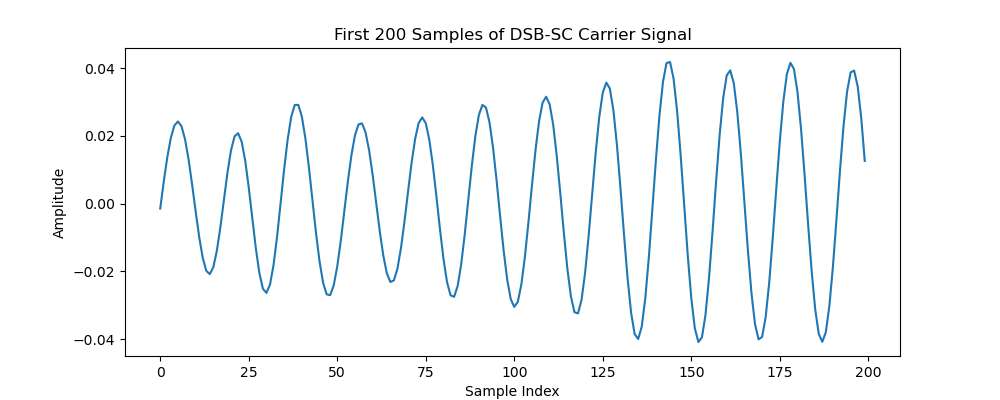
\includegraphics[width=1.2\textwidth]{assignment5b.png} % Include the figure
	\caption{First 200 Samples of DSB-SC Carrier Signal in Time-Domain}
	\label{fig:block}
\end{figure}

\begin{figure}[H] % [H] forces the figure to be placed exactly where it appears in the text
	\centering % Horizontally center the figure
	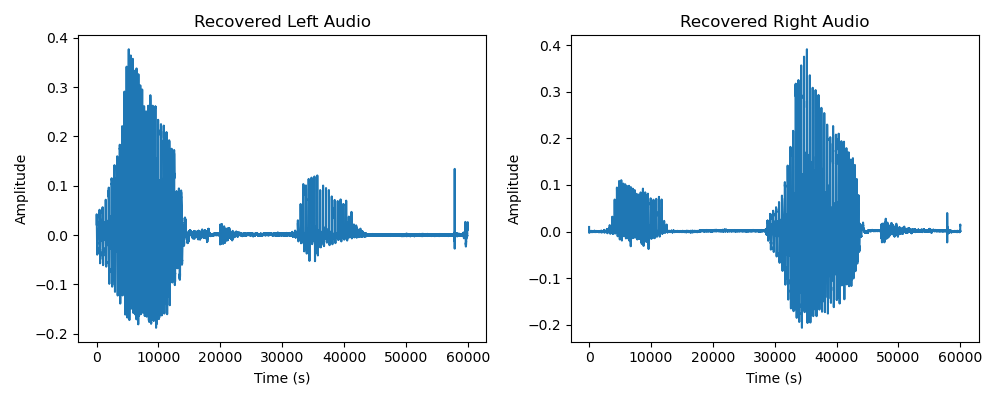
\includegraphics[width=1.2\textwidth]{assignment5c.png} % Include the figure
	\caption{Recovered Left+Right Signal in Time-Domain}
	\label{fig:block}
\end{figure}

\section{Assignment 6}

\begin{lstlisting}[language=Python]
	import numpy as np
	import matplotlib.pyplot as plt
	from scipy.io import wavfile
	from scipy.signal import butter, filtfilt, resample_poly, hilbert
	import adi
	
	# Set SDR parameters
	sdr_carrier_freq = 96.9e6  # Choose a local FM station frequency
	sdr_rx_gain = 50.0  # Rx gain (Adjust based on signal strength)
	M = 15  # Upsampling factor
	fs_audio = 44100  # Audio sampling rate (Hz)
	fs = M * fs_audio  # PlutoSDR sampling rate (Hz)
	N = 900000  # Close to maximum buffer size (1.4 sec per buffer)
	
	# Create PlutoSDR object
	sdr = adi.Pluto("ip:192.168.2.1")
	
	# Configure common settings
	sdr.sample_rate = int(fs)
	sdr.gain_control_mode_chan0 = 'manual'
	
	# Configure Rx
	sdr.rx_lo = int(sdr_carrier_freq)
	sdr.rx_rf_bandwidth = int(fs)
	sdr.rx_buffer_size = int(N)  # Buffer size for Rx samples
	sdr.rx_hardwaregain_chan0 = sdr_rx_gain  # Adjust Rx gain (0 to 74.5 dB)
	
	# Clear buffer before capturing data
	for _ in range(3):
	sdr.rx()
	
	# Capture multiple frames (about 5 sec of audio)
	num_frames = 4
	raw_data = []
	for _ in range(num_frames):
	temp = sdr.rx()
	raw_data = np.concatenate([raw_data, temp])
	raw_data = np.array(raw_data) * 2**-14  # Scale samples to (-1,1)
	
	# Apply 53 kHz LPF to remove out-of-band noise
	Nfilt_rf = 11
	cutoff_rf = 53e3
	b_LPF_rf, a_LPF_rf = butter(Nfilt_rf, cutoff_rf / (fs / 2), btype='low')
	filtered_data = filtfilt(b_LPF_rf, a_LPF_rf, raw_data)
	
	# Extract phase from the complex signal
	phase_rx = np.unwrap(np.angle(filtered_data))
	
	# Compute the FM demodulated message signal
	mRx = (phase_rx[1:] - phase_rx[:-1]) * fs / (2 * np.pi * 75e3)
	mRx = np.append(mRx, mRx[-1])  # Append a zero to match the original length
	
	# Extract Audio Components
	# Low-pass filter for L+R audio (0-15 kHz)
	Nfilt_audio = 9
	cutoff_audio = 15e3
	b_LPF_audio, a_LPF_audio = butter(Nfilt_audio, cutoff_audio / (fs / 2), btype='low')
	L_plus_R = filtfilt(b_LPF_audio, a_LPF_audio, mRx)
	
	# Narrowband filter for pilot tone (19 kHz)
	Nfilt_band = 5
	cutoff_band_pilot = [18e3, 20e3]
	b_narrow, a_narrow = butter(Nfilt_band, np.array(cutoff_band_pilot) / (fs / 2), btype='band')
	pilot_rx = filtfilt(b_narrow, a_narrow, mRx)
	
	# Band-pass filter for DSB-SC carrier (38 kHz)
	cutoff_band_dsb = [23e3, 53e3]
	b_BPF, a_BPF = butter(Nfilt_band, np.array(cutoff_band_dsb) / (fs / 2), btype='band')
	DSB_carrier_rx = filtfilt(b_BPF, a_BPF, mRx)
	
	# Extract phase of the recovered pilot using Hilbert transform
	pilot_phase = np.unwrap(np.angle(hilbert(pilot_rx)))
	
	# Double the phase to obtain the DSB-SC carrier
	DSB_carrier_phase = 2 * pilot_phase
	
	# Recover the difference signal (L-R)
	L_minus_R = DSB_carrier_rx * np.cos(DSB_carrier_phase) * 2
	
	# Recover Left and Right channels
	L_audio = (L_plus_R + L_minus_R) / 2
	R_audio = (L_plus_R - L_minus_R) / 2
	
	# Downsample audio back to 44.1 kHz
	L_audio_downsampled = resample_poly(L_audio, 1, M)
	R_audio_downsampled = resample_poly(R_audio, 1, M)
	
	# Save the recovered mono and stereo audio as WAV files
	from scipy.io.wavfile import write
	
	# Mono Audio (L+R)
	mono_audio = (L_audio_downsampled + R_audio_downsampled) / 2
	mono_audio_int16 = (mono_audio * 32767).astype(np.int16)  # Convert to 16-bit PCM
	write("fm_mono.wav", int(fs_audio), mono_audio_int16)
	
	# Stereo Audio (L, R)
	stereo_demod = np.column_stack((L_audio_downsampled, R_audio_downsampled))
	stereo_demod_int16 = (stereo_demod * 32767).astype(np.int16)  # Convert to 16-bit PCM
	write("fm_stereo.wav", int(fs_audio), stereo_demod_int16)
	
\end{lstlisting}

\end{document}